%%%%%%%%%%%%%%%%%%%%%%%%%%%%%%%%%%%%%%%%%%%%%%%%%%%%%%%%%%%%%%%%%%%%%%%%%%%%%%%%
% Template for USENIX papers.
%
% History:
%
% - TEMPLATE for Usenix papers, specifically to meet requirements of
%   USENIX '05. originally a template for producing IEEE-format
%   articles using LaTeX. written by Matthew Ward, CS Department,
%   Worcester Polytechnic Institute. adapted by David Beazley for his
%   excellent SWIG paper in Proceedings, Tcl 96. turned into a
%   smartass generic template by De Clarke, with thanks to both the
%   above pioneers. Use at your own risk. Complaints to /dev/null.
%   Make it two column with no page numbering, default is 10 point.
%
% - Munged by Fred Douglis <douglis@research.att.com> 10/97 to
%   separate the .sty file from the LaTeX source template, so that
%   people can more easily include the .sty file into an existing
%   document. Also changed to more closely follow the style guidelines
%   as represented by the Word sample file.
%
% - Note that since 2010, USENIX does not require endnotes. If you
%   want foot of page notes, don't include the endnotes package in the
%   usepackage command, below.
% - This version uses the latex2e styles, not the very ancient 2.09
%   stuff.
%
% - Updated July 2018: Text block size changed from 6.5" to 7"
%
% - Updated Dec 2018 for ATC'19:
%
%   * Revised text to pass HotCRP's auto-formatting check, with
%     hotcrp.settings.submission_form.body_font_size=10pt, and
%     hotcrp.settings.submission_form.line_height=12pt
%
%   * Switched from \endnote-s to \footnote-s to match Usenix's policy.
%
%   * \section* => \begin{abstract} ... \end{abstract}
%
%   * Make template self-contained in terms of bibtex entires, to allow
%     this file to be compiled. (And changing refs style to 'plain'.)
%
%   * Make template self-contained in terms of figures, to
%     allow this file to be compiled.
%
%   * Added packages for hyperref, embedding fonts, and improving
%     appearance.
%
%   * Removed outdated text.
%
%%%%%%%%%%%%%%%%%%%%%%%%%%%%%%%%%%%%%%%%%%%%%%%%%%%%%%%%%%%%%%%%%%%%%%%%%%%%%%%%

\documentclass[letterpaper,twocolumn,10pt]{article}
\usepackage{usenix-2020-09}

% to be able to draw some self-contained figs
\usepackage{tikz}
\usepackage{amsmath}
\usepackage{subfig}

% use for decent code formatting
\usepackage{inconsolata}
\usepackage[outputdir=build]{minted}


% notes for different people
\newcommand{\tg}[1]{\ifisdraft{\color{blue}[#1 -- Todd]}\fi}

%-------------------------------------------------------------------------------
\begin{document}
%-------------------------------------------------------------------------------

%don't want date printed
\date{}

% make title bold and 14 pt font (Latex default is non-bold, 16 pt)
\title{\Large \bf Formatting Submissions for a USENIX Conference:\\
  An (Incomplete) Example}

%for single author (just remove % characters)
\author{
{\rm Your N.\ Here}\\
Your Institution
\and
{\rm Second Name}\\
Second Institution
% copy the following lines to add more authors
% \and
% {\rm Name}\\
%Name Institution
} % end author

\maketitle

%-------------------------------------------------------------------------------
\begin{abstract}
%-------------------------------------------------------------------------------
Your abstract text goes here. Just a few facts. Whet our appetites.
Not more than 200 words, if possible, and preferably closer to 150.
\end{abstract}


%-------------------------------------------------------------------------------
\section{Introduction}
%-------------------------------------------------------------------------------
- Todd
{\tt this is some monospace stuff.}

A paragraph of text goes here. Lots of text. Plenty of interesting
text. Text text text text text text text text text text text text text
text text text text text text text text text text text text text text
text text text text text text text text text text text text text text
text text text text text text text.
More fascinating text. Features galore, plethora of promises.

%-------------------------------------------------------------------------------
\section{Package Managers}
%-------------------------------------------------------------------------------
-- Todd
Background on different kinds of package managers, highlighting commonalities and differences (e.g. conda, Go, system package managers). Introduce Spack and explain how it is different from others.

%-------------------------------------------------------------------------------
\section{Spack}
%-------------------------------------------------------------------------------
-- Greg
\subsection{Spec Syntax}

\subsection{Package DSL}

\subsection{Concretization}
- user configuration
- CLI arguments
- package constraints

\subsection{Dependency Model}
Discuss the software dependency model used in Spack and the future roadmap. Introduce concepts like variants, ABI compatibility etc. that are either implicit or disregarded by other package managers.


%-------------------------------------------------------------------------------
\section{Answer Set Programming}
%-------------------------------------------------------------------------------
-- Todd
Background on ASP solvers

%-------------------------------------------------------------------------------
\section{Modeling Software Dependencies with ASP}
%-------------------------------------------------------------------------------
-- Max
Time to explain concretize.lp

\subsection{Simple Examples}
- avoiding cycles
- specializing BLAS
- conditional variants -- ROCM/CUDA

- Generalized Condition Handling
  - examples of: conflicts, virtuals, dependencies, variants

\section{Reusing installed packages}
Max / Todd
\subsection{reuse in nix, guix, conan, and old spack}
- by hash

\subsection{optimizing for reuse}
- reuse of half the generalized condition
- Reusing built dependencies

\subsection{optimizing for reuse}
- architecting optimization criteria for builds vs. reuse

%-------------------------------------------------------------------------------
\section{Error Handling for Unsolvable Problems}
%-------------------------------------------------------------------------------
Greg
How do we want to perform error handling?


%-------------------------------------------------------------------------------
\section{Performance Results}
%-------------------------------------------------------------------------------
Sergei


\subsection{Solve timings for all packages}


\begin{figure*}[htb]

    \centering
    \subfloat[][Ground times]{
    \label{subfig:cdf_quartz_ground}
        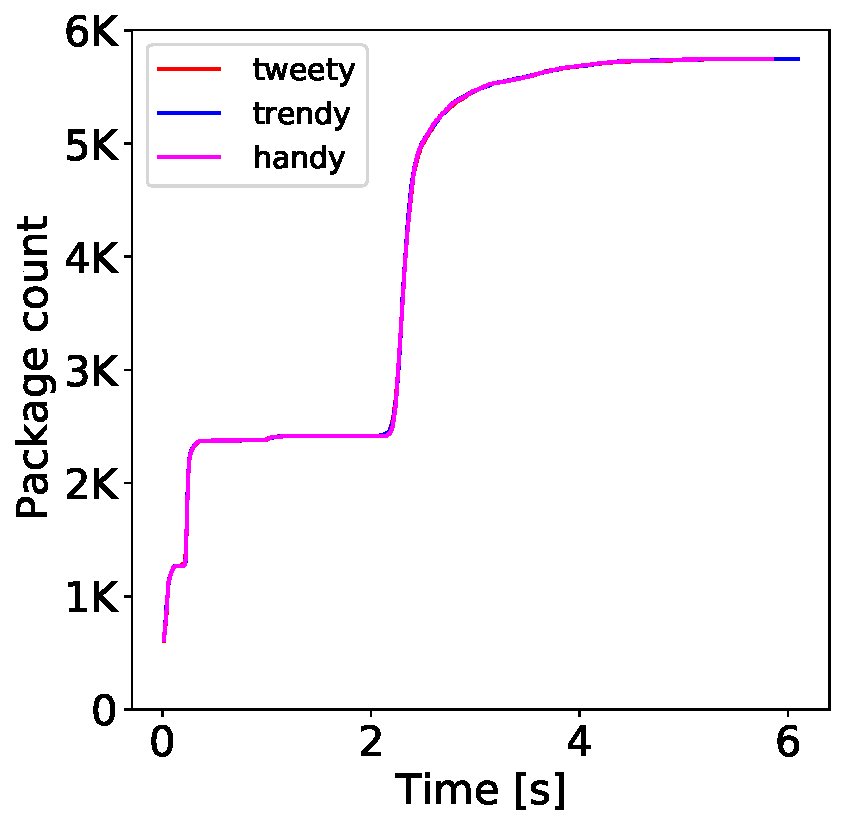
\includegraphics[width=\perfsubfigwidth\textwidth]{figures/perf/cdf_quartz_ground_fig.pdf}
    }\hfill%
    \subfloat[][Solve times]{
    \label{subfig:cdf_quartz_solve}
        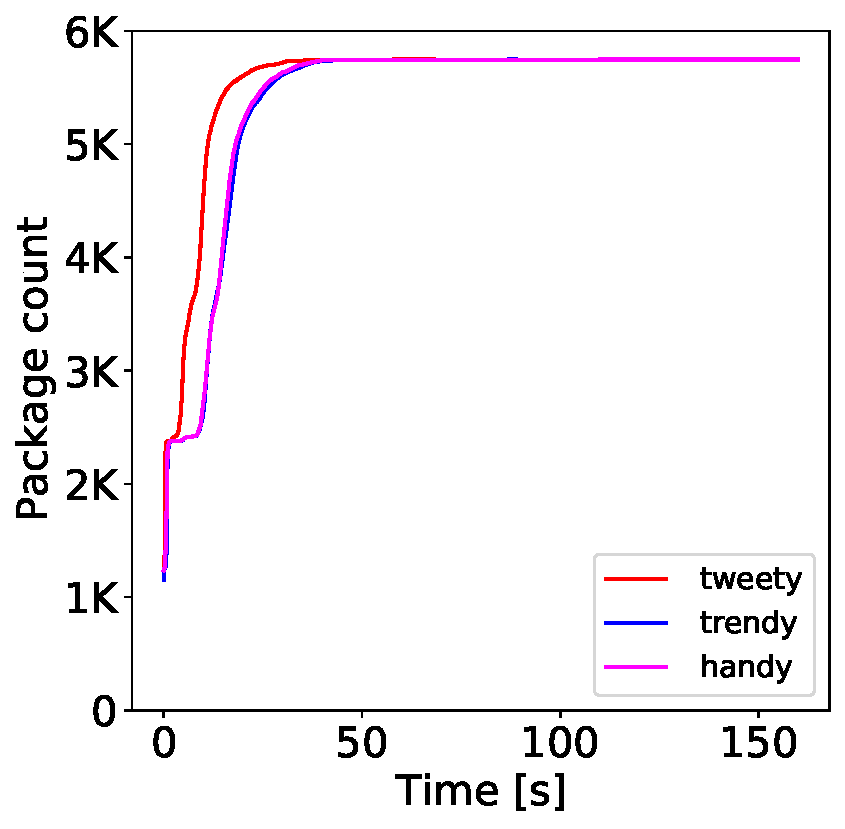
\includegraphics[width=\perfsubfigwidth\textwidth]{figures/perf/cdf_quartz_solve_fig.pdf}
    }\hfill%
    \subfloat[][Full solving times]{
    \label{subfig:cdf_quartz_full}
        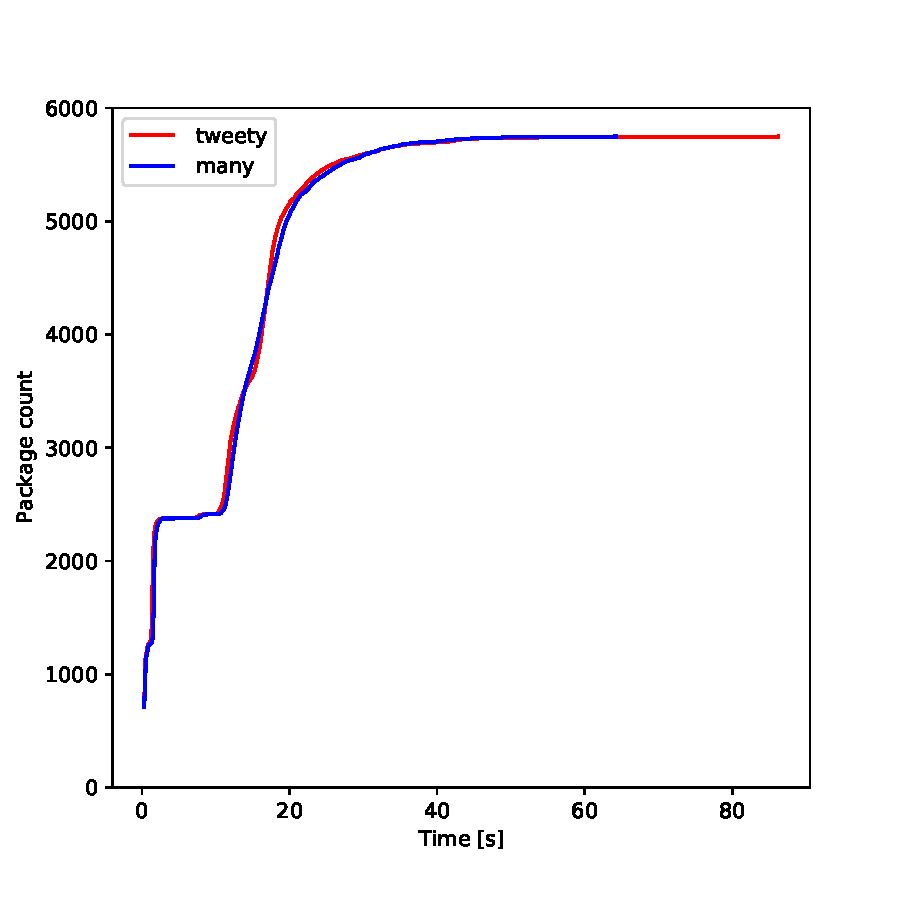
\includegraphics[width=\perfsubfigwidth\textwidth]{figures/perf/cdf_quartz_total_fig.pdf}
    }
    \caption{Cumulative distribution of solve times across all packages on the Quartz machine.}
    \label{fig:cdf_quartz}

\end{figure*}



\begin{figure*}[htb]

    \centering
    \subfloat[][Load times]{
    \label{subfig:cdf_lassen_load}
        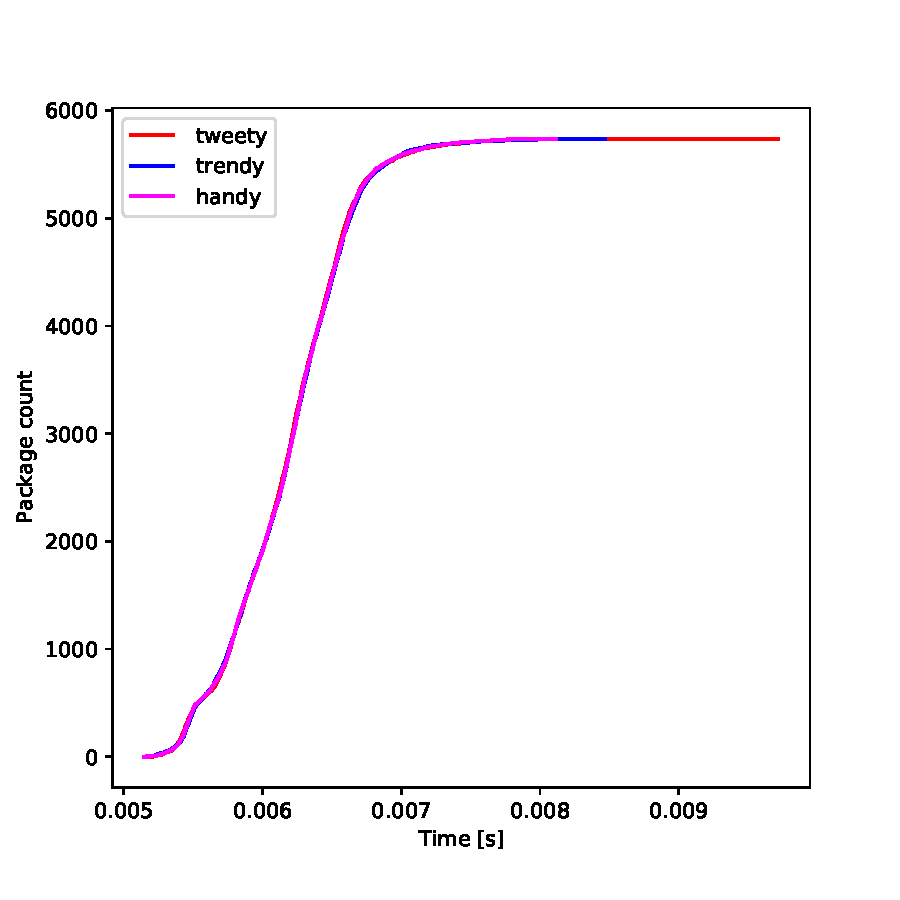
\includegraphics[width=0.32\textwidth]{figures/perf/cdf_lassen_load_fig.pdf}
    }\hfill%
    \subfloat[][Solve times]{
    \label{subfig:cdf_lassen_solve}
        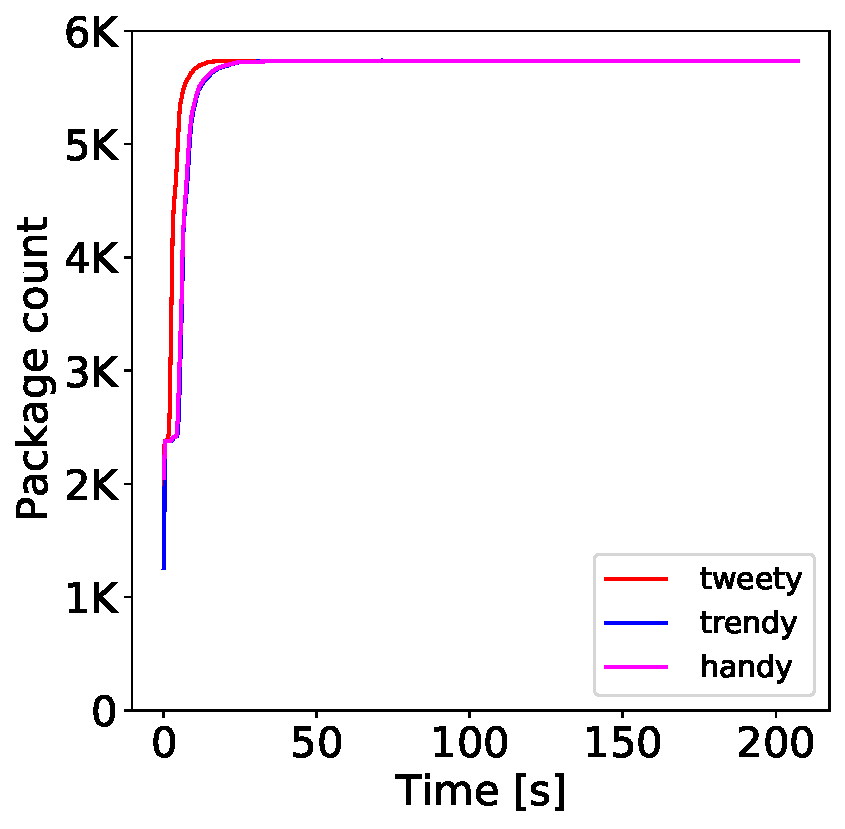
\includegraphics[width=0.32\textwidth]{figures/perf/cdf_lassen_solve_fig.pdf}
    }\hfill%
    \subfloat[][Full solving times]{
    \label{subfig:cdf_lassen_full}
        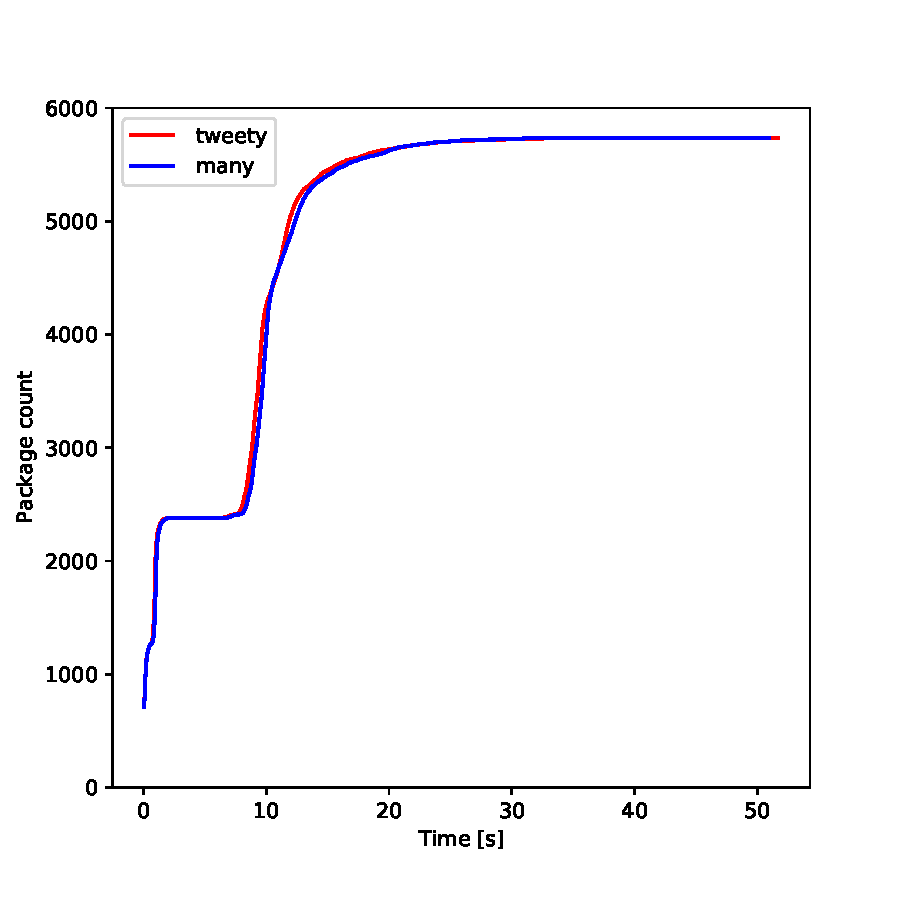
\includegraphics[width=0.32\textwidth]{figures/perf/cdf_lassen_total_fig.pdf}
    }
    \caption{Cumulative distribution of solve times across all packages on the Lassen machine.}
    \label{fig:cdf_quartz}

\end{figure*}



\begin{figure*}[htb]

    \centering
    \subfloat[][Ground times]{
    \label{subfig:deps_quartz_load}
        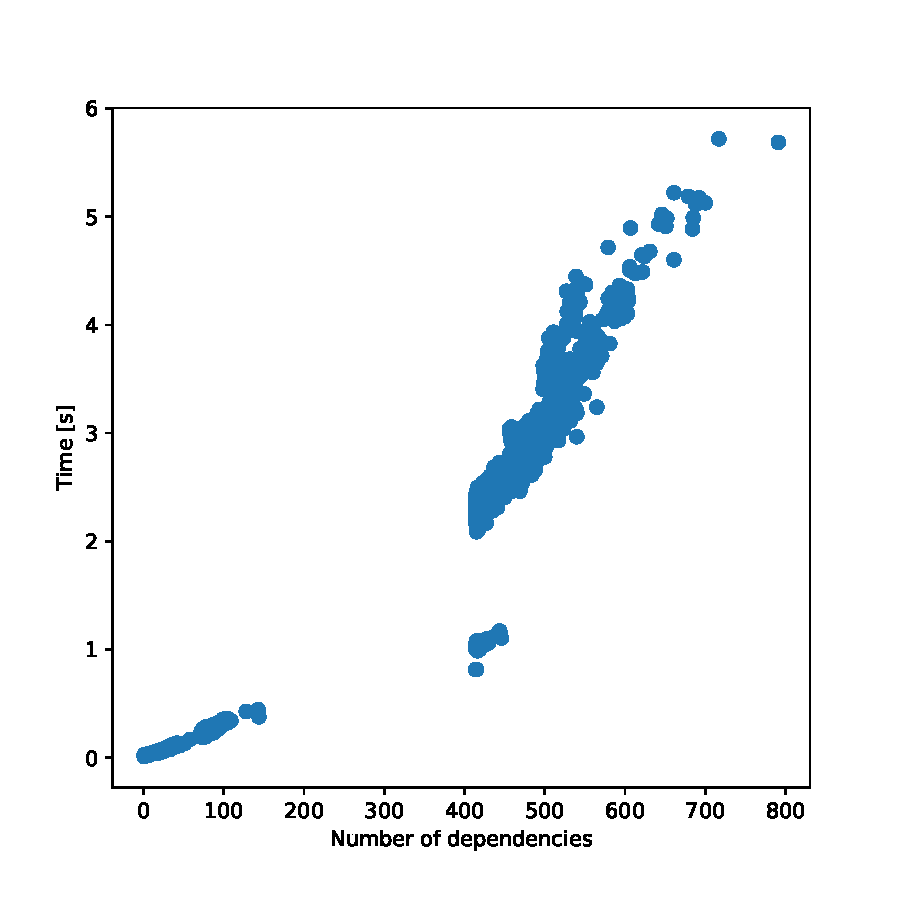
\includegraphics[width=0.32\textwidth]{figures/perf/deps_quartz_ground_fig.pdf}
    }\hfill%
    \subfloat[][Solve times]{
    \label{subfig:deps_quartz_solve}
        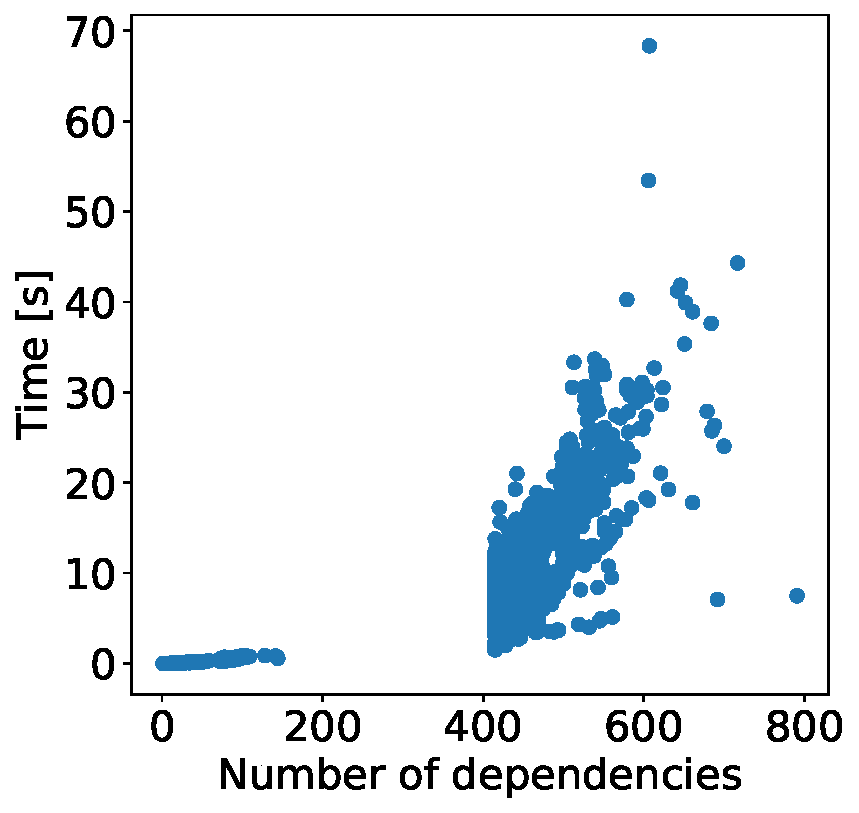
\includegraphics[width=0.32\textwidth]{figures/perf/deps_quartz_solve_fig.pdf}
    }\hfill%
    \subfloat[][Full solving times]{
    \label{subfig:deps_quartz_full}
        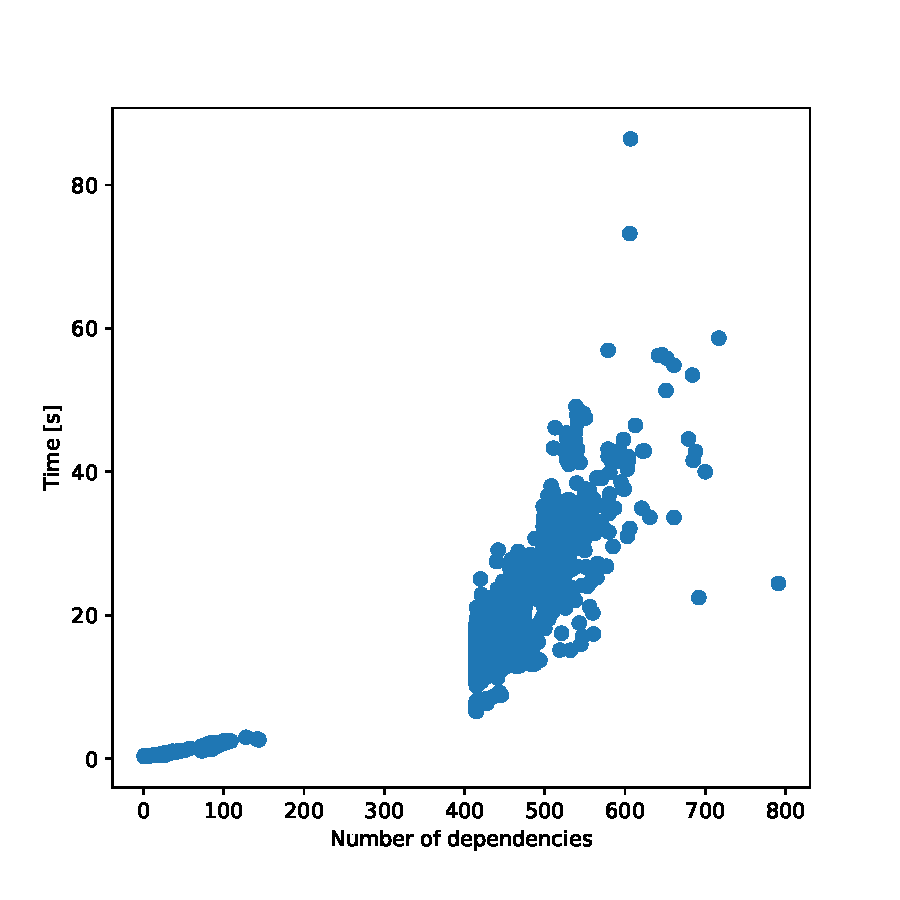
\includegraphics[width=0.32\textwidth]{figures/perf/deps_quartz_total_fig.pdf}
    }
    \caption{Solve times vs. number of dependent packages across all packages on the Quartz machine.}
    \label{fig:deps_quartz}

\end{figure*}



\begin{figure*}[htb]

    \centering
    \subfloat[][Ground times]{
    \label{subfig:deps_lassen_load}
        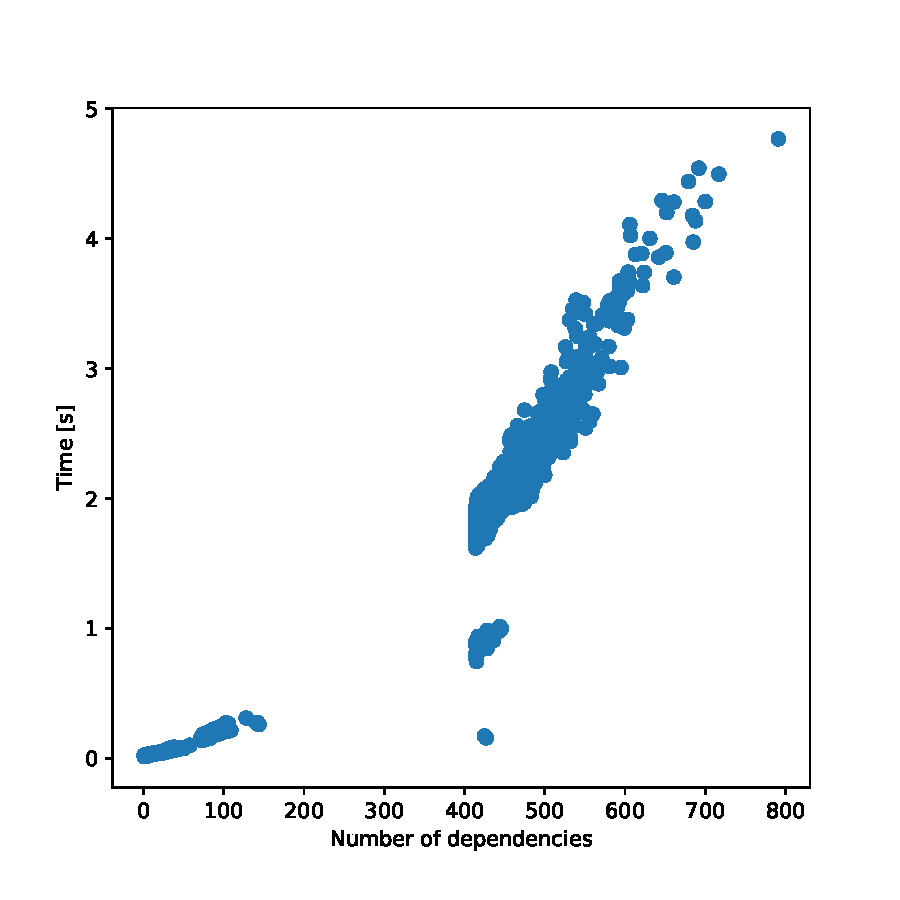
\includegraphics[width=\perfsubfigwidth\textwidth]{figures/perf/deps_lassen_ground_fig.pdf}
    }\hfill%
    \subfloat[][Solve times]{
    \label{subfig:deps_lassen_solve}
        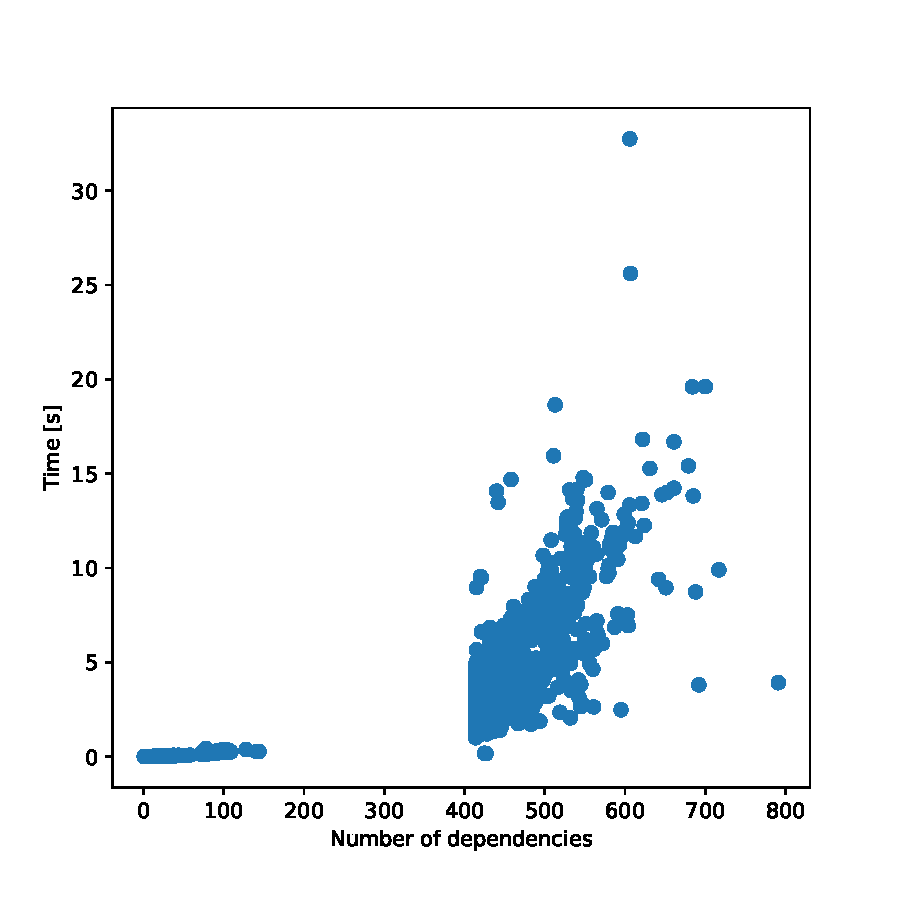
\includegraphics[width=\perfsubfigwidth\textwidth]{figures/perf/deps_lassen_solve_fig.pdf}
    }\hfill%
    \subfloat[][Full solving times]{
    \label{subfig:deps_lassen_full}
        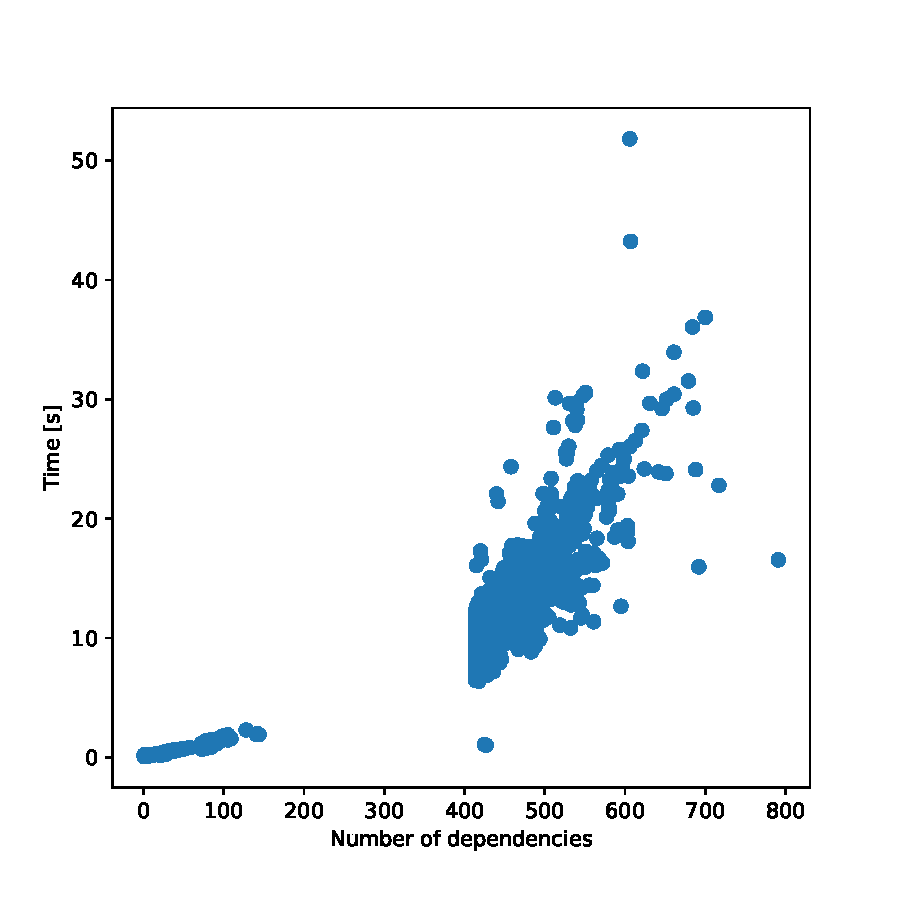
\includegraphics[width=\perfsubfigwidth\textwidth]{figures/perf/deps_lassen_total_fig.pdf}
    }
    \caption{Solve times vs. number of dependent packages across all packages on the Lassen machine.}
    \label{fig:deps_lassen}

\end{figure*}


- Time vs. number of dependnecies
- other properties?
- --single-shot vs. no single-shot?
- different tactics?

\subsection{Solve timings for all packages with reuse}
- scaling repo size


How is the ASP based solver performing?

\section{Conclusions}
- TBD
A paragraph of text goes here. Lots of text. Plenty of interesting
text. Text text text text text text text text text text text text text
text text text text text text text text text text text text text text
text text text text text text text text text text text text text text
text text text text text text text.
More fascinating text. Features galore, plethora of promises.

%-------------------------------------------------------------------------------
\section*{Acknowledgments}
%-------------------------------------------------------------------------------
The USENIX latex style is old and very tired, which is why
there's no \textbackslash{}acks command for you to use when
acknowledging. Sorry.

%-------------------------------------------------------------------------------
\section*{Availability}
%-------------------------------------------------------------------------------

USENIX program committees give extra points to submissions that are
backed by artifacts that are publicly available. If you made your code
or data available, it's worth mentioning this fact in a dedicated
section.

%-------------------------------------------------------------------------------
% References
%-------------------------------------------------------------------------------
{
   \footnotesize
   \bibliographystyle{abbrv}
   \bibliography{\jobname}
}

%%%%%%%%%%%%%%%%%%%%%%%%%%%%%%%%%%%%%%%%%%%%%%%%%%%%%%%%%%%%%%%%%%%%%%%%%%%%%%%%
\end{document}
%%%%%%%%%%%%%%%%%%%%%%%%%%%%%%%%%%%%%%%%%%%%%%%%%%%%%%%%%%%%%%%%%%%%%%%%%%%%%%%%

%%  LocalWords:  endnotes includegraphics fread ptr nobj noindent
%%  LocalWords:  pdflatex acks
